%
% burgerintro.tex
%
% (c) 2018 Prof Dr Andreas Müller, Hochschule Rapperswil
%
\section{Die Gleichung von Burgers\label{section:burgersallg}}
Die Gleichung von Burgers ist ein prototypisches Beispiel einer nichtlinearen
partiellen Differentialgleichung, an dem sich viele für nichtlineare
Differentialgleichungen typische Phänomene in einer einfachen Situation
studieren lassen.
Zum Beispiel tritt bei einigen numerischen Lösungsverfahren für die
Gleichung von Burgers häufig eine Instabilität auf, die man 
Computational Mode nennt.
Natürlich sind Tricks entwickelt worden, mit diesem Problem fertig
zu werden.
Der zuvor für die Wärmeleitungsgleichung untersuchte Ansatz, ein
Lösungsverfahren mit Hilfe von Machine Learning zu konstrieren birgt
das Potential, den Computational Mode von Anfang an zu vermeiden.
Das Verfahren kann ja nur lernen, was auch in den Trainingsdaten
erkennbar ist, und wir können sicherstellen, dass die Trainingsdaten
keine Lösungen enthalten, die Anzeichen des Computational Mode beinhalten.

In diesem Abschnitt sammeln wir ein paar Fakten über die Gleichung 
von Burgers und den Computational mode.
In einem späteren Abschnitt werden wir diese Informationen dazu
verwenden, um Trainingsdaten zu erzeugen.

\subsection{Nichtlineare Transportgleichung\label{subsection:nichtlineare}}
Die Gleichung von Burgers in der Form
\begin{equation}
\frac{\partial u}{\partial t} + u\frac{\partial u}{\partial x}=0
\qquad\text{mit Anfangsbedingung}\qquad
u(0,x) = u_0(x)
\label{burgers:transport}
\end{equation}
modelliert ein nichtlneares Transportproblem.
Die Gleichung~\eqref{burgers:transport} ist eine quasilineare partielle
Differentialgleichung erster Ordnung, die mit der Methode der
Charakteristiken \cite{burgers:pde} gelöst werden kann.
Die Charakteristiken-Gleichungen sind
\begin{align*}
t'(s)&=1
\\ 
x'(s)&=u
\\
u'(s)&=0
\end{align*}
Aus der ersten Gleichung leitet man ab, tdass $s=t$.
Die dritte Gleichung besagt, dass $u$ entlang einer Charakteristik konstant
ist, also $u(s)=u_0$.
Die zweite Gleichung besagt dann, dass die im Punkt $(0,x_0,u_0(x_0))$
beginnende Charakteristik eine Gerade mit $x(t)=x_0 + u_0(x_0)t$ ist.

\begin{figure}
\centering
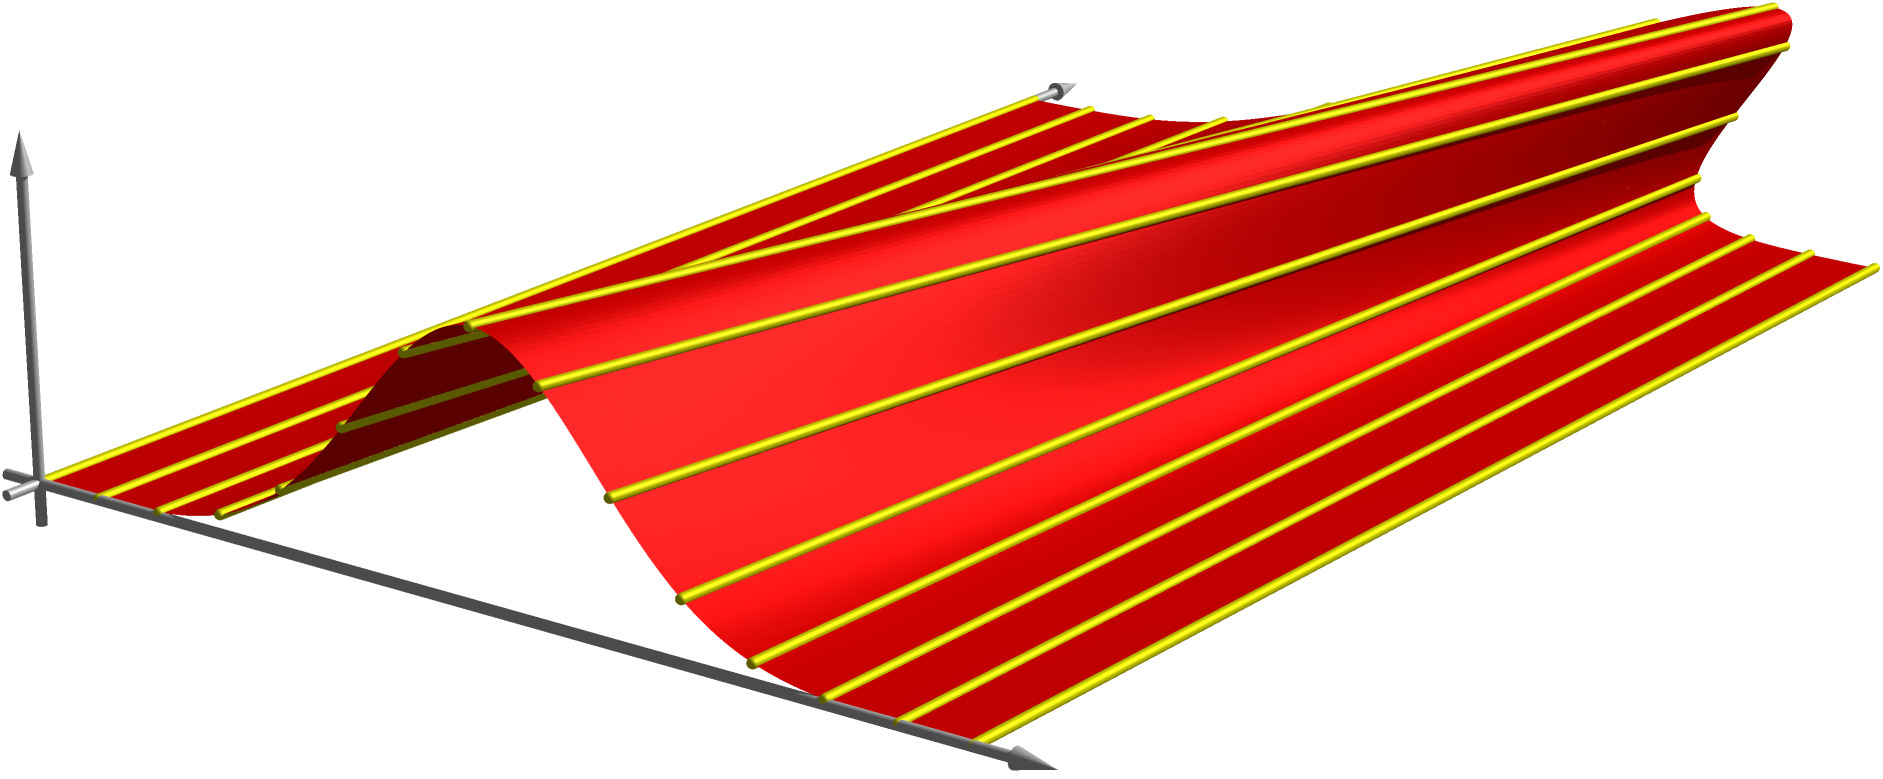
\includegraphics[width=\hsize]{learning/welle.jpg}
\caption{Lösung der Gleichung von Burgers mit Hilfe der Methode
der Charakteristiken.
Die Lösungsfläche ist darstellbar als eine Schar von Geraden (gelb).
\label{burgers:charloesung}}
\end{figure}
Die Abbildung~\ref{burgers:charloesung} 
zeigt eine Lösung mit einer Gauss-Verteilung als Anfangsbedingung.
Es ist offensichtlich, dass die gezeigte Fläche früher oder später nicht
mehr Graph einer Funktion $u(x,y)$ sein kann.
Es entwickelt sich eine Sprungstelle, die Gleichung von Burgers ist
ein Modell für eine Schockwelle.
Man kann insbesondere nicht erwarten, dass die Gleichung von Burgers
für beliebige Zeiten $t$ eine glatte Lösung hat, selbst wenn die
Anfangsbedingungen glatt waren.
Man muss sich mit einer schwachen Lösung begnügen.
Dies hat sowohl auf numerische Lösungsverfahren Auswirkungen wie auch
auf das Problem, Trainingsdaten für auf Machine Learning basierenden
Lösungsalgorithmus zu erzeugen.

\subsection{Erhaltungssatz\label{subsection:erhaltungssatz}}
Die Gleichung von Burgers kann man auch in der Form
\begin{equation}
\frac{\partial u}{\partial t}
+
\frac{\partial}{\partial x} \frac{u^2}{2}
=
0
\label{burgers:erhaltungssatz}
\end{equation}
formulieren.
Dies ist ein Spezialfall der allgemeineren Gleichung
\begin{equation}
\frac{\partial u}{\partial t}
+
\frac{\partial }{\partial x} F(u)
=
0
\label{burgers:conservationlaw}
\end{equation}
mit $F(u)=\frac12u^2$.
Man nennt 
\eqref{burgers:conservationlaw}
einen Erhaltungssatz.
Diese Betrachtungsweise erlaubt, die Bewegung von Sprungstellen besser
zu verstehen.

Die Differentialgleichung~\eqref{burgers:conservationlaw} kann auch
in der Form
\[
\frac{\partial u}{\partial t}
+
\frac{\partial }{\partial x} F(u)
=
\begin{pmatrix}
\frac{\partial}{\partial t}
\\
\frac{\partial}{\partial x}
\end{pmatrix}
\begin{pmatrix}t\\F(u)\end{pmatrix}
=
\nabla\cdot 
\begin{pmatrix}t\\F(u)\end{pmatrix}
=0
\]
schreiben.
Darauf ist aber der Satz \ref{skript:wegunabhaengigkeit} anwendbar.
Er besagt, dass Integrale
\begin{align}
\oint_\gamma(
F(u)\,dt
-
u\,dx
)
&=
\int_D \frac{\partial u}{\partial t}+\frac{\partial}{\partial x}F(u)\,dx\,dy
=
0
\label{burgers:integral}
\end{align}
über geschlossene Wege $\gamma$ verschwinden.

\subsection{Hugoniot-Rankine-Bedingungen\label{subsection:hugnoniot}}
\begin{figure}
\centering
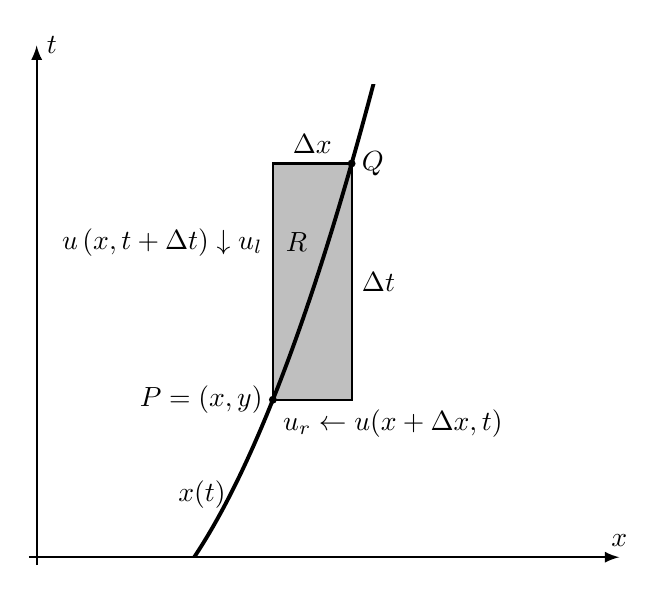
\begin{tikzpicture}[>=latex,thick]
\fill[color=gray!50] (3,2)--(4,2)--(4,5)--(3,5)--cycle;
\node at (3.3,4.0) {$R$};
\draw[->] (-0.1,0)--(7.4,0) coordinate[label={$x$}];
\draw[->] (0,-0.1)--(0,6.5) coordinate[label={right:$t$}];
\fill (3,2) circle[radius=0.05];
\node at (3,2) [left] {$P=(x,y)$};
\fill (4,5) circle[radius=0.05];
\node at (4,5) [right] {$Q$};
\draw (3,2)--(4,2)--(4,5)--(3,5)--cycle;
\node at (3.5,5) [above] {$\Delta x$};
\node at (4,3.5) [right] {$\Delta t$};
\begin{scope}
\clip (0,0) rectangle (7,6.0);
\draw[line width=1.4pt] plot[domain=2:5,samples=100] ({\x},{0.5*\x*\x -0.5*(\x)-1});
\end{scope}
\node at (3,4) [left] {$\begin{matrix}u(x,t+\Delta t)\\\downarrow\\u_l\end{matrix}$};
\node at (3,2) [below right] {$u_r\leftarrow u(x+\Delta x,t)$};
\node at (2.1,0.8) {$x(t)$};
\end{tikzpicture}
\caption{Herleitung der Hugoniot-Rankine-Bedingung für die Bewegung einer
Sprungstelle der Lösung eines Erhaltungssatzes.
\label{burgers:hugoniot}}
\end{figure}
In Abschnitt~\ref{subsection:nichtlineare} haben wir gesehen, dass Lösungen
der Gleichung von Burgers Sprungstellen entwickeln.
Die Formulierung als Erhaltungssatz in
Abschnitt~\ref{subsection:erhaltungssatz} 
soll uns jetzt erlauben, die Bewegung solcher Sprungstellen zu beschreiben.

Sie also $u(t,x)$ eine Lösung fast überall der Gleichung von Burgers mit
einer Sprungstelle, die sich entlangt der Kurve $x(t)$ bewegt.
Dazu berechnen wir das Wegintegral \eqref{burgers:integral} über den Rand
des Rechtecks mit den Ecken $(x,y)$ und $(x+\Delta x, y+\Delta y)$.
Wir benötigen die Grenzwerte
\[
\begin{aligned}
u_l &= \lim_{\Delta t\to 0+} u(t+\Delta t,x)
&&\text{und}&
u_r &= \lim_{\Delta x\to 0+} u(t,x+\Delta x).
\end{aligned}
\]
Damit können wir das Wegintegral approximieren als
\begin{align}
\int_{\partial R}(u\,dx -F(u)\,dt)
&=
0
\notag
\\
u(t+\Delta t,x)
\Delta x
-
F(u(t+\Delta t,x))
\Delta t
&=
u(t,x+\Delta x) \Delta x
-
F(u(t,x+\Delta x)) \Delta t
\notag
\\
\Delta x
(
u(t+\Delta t,x)
-
u(t,x+\Delta x)
)
&=
\Delta t
(F(u(t+\Delta t,x))
-
F(u(t,x+\Delta x))
)
\notag
\\
\intertext{Oder nach Grenzübergang $\Delta t\to 0$ und $\Delta x\to 0$}
\dot x(t)\, (u_l-u_r) &= F(u_l) - F(u_r).
\label{burgers:hugoniot-rankine}
\end{align}
Die Geschwindigkeit, mit der sich die Sprungstelle bewegt, hängt also 
von den Werten von $u(t,x)$ auf beiden Seiten der Sprungstelle ab.
Dies sind die {\em Hugoniot-Rankine-Bedingungen}.
Wir werden sie Abschnitt~\ref{burgers:training} verwenden, um Trainingsdaten
für Sprungstellen der Lösung zu erzeugen.
\index{Hugoniot-Rankine-Bedingungen}
\index{Rankine-Hugoniot-Bedingungen}

Im Fall der Gleichung von Burgers ist $F(u)=\frac12u^2$.
Die Hugoniot-Rankine-Bedingung wird dann zu
\begin{equation}
\dot x(t)\, (u_l-u_r) = \frac12 (u_l^2-u_r^2)
\qquad\Rightarrow\qquad
\dot x(t)
=
\frac12 (u_l+u_r).
\end{equation}
Eine Sprungstelle der Gleichung von Burgers bewegt sich also immer
mit der Geschwindigkeit, die dem Mittelwert der $u$-Werte auf
beiden Seiten der Sprungstelle entspricht.

\subsection{Numerische Lösungen und Computational mode}
Bei der numerischen Lösung der Gleichung von Burgers tritt erschwehrend ein
Computational Mode auf.
Ziel dieses Abschnittes ist, die Herkunft des Computational Mode zu erklären
und an einem numerischen Experiment zu illustrieren, wie er auch bei
der Gleichung von Burgers zu Instabilität bei der numerischen
Lösung führen kann.

\subsubsection{Ein einfacheres Beispiel}
Wir betrachten die gewöhnliche Differentialgleichung
\begin{equation}
\frac{du}{dx}=0.
\label{burgers:konstant}
\end{equation}
Die einzigen Lösungen dieser Differentialgleichungen sind die konstanten
Funktionen.
Wir würden also erwarten, dass auch ein numerisches Verfahren nur
die konstanten Funktionen als Lösungen hervorbringen würde.

Wir beginnen mit einer Diskretisierung $x_i=ih$, $i\in\mathbb N$, und
versuchen eine Lösung $u_i= u(x_i)$ zu konstruieren.
Die Ableitung wird durch Differenzenquotienten approximiert, dies
führt auf die Gleichungen
\begin{equation}
0
=
\frac{du(x_i)}{dx}
=
\frac{u_{i+1}-u_{i}}{x_{i+1}-x_{i}} = \frac{u_{i+1}-u_i}{h},
\label{burgers:diffquot}
\end{equation}
was gleichbedeutend ist mit der Rekursionsgleichung
\[
u_{i+1} = u_{i}.
\]
Diese besagt natürlich nichts anderes als dass wie erwartet
die Lösungsfunktion konstant sein muss.

Das Problem dieses Beispiel ist jedoch, dass der Differenzenquotient
\eqref{burgers:diffquot} gar nicht repräsentativ ist für eine Ableitung
an der Stelle $x_i$, sondern eher für $u'(x_i+\frac12h)$.
Ein symmetrischer Differenzenquotient 
\[
u'(x_i)
\simeq
\frac{u_{i+1}-u_{i-1}}{x_{i+1}-x_{i-1}}=\frac{u_{i+1}-u_{i-1}}{2h}=0
\]
ist zutreffender, führt aber auf die Rekursionsgleichung
\[
u_{i+1}=u_{i-1}.
\]
Diese hat zwei linear unabhängige Lösungen, die Gleichungen besagen
nämlich nur, dass alle geraden Werte $u_{2i}=u_0$ und alle ungeraden
$u_{2i+1}=u_1$ sind, diese beiden Werte können aber durchaus verschieden
sein.
Der Versuch, den Differenzenquotienten genauer wiederzugeben hat 
zusätzliche numerische Lösungen hervorgebracht, die nichts mit Lösungen
der Differentialgleichung zu tun haben.

\subsubsection{Differentialgleichung für die Exponentialfunktion}
Das Beispiel~\eqref{burgers:konstant} war insofern künstlich, als auf der
rechten Seite die Werte von $u$ gar nicht gebraucht wurden und daher das
Argument, der Differenzenquotient~\eqref{burges:diffquote} können nicht
mit der rechten Seite verglichen werde, nicht wirklich stichhaltig ist.
Dies ändert sich mit der Gleichung
\begin{equation}
\frac{du}{dx} = -u.
\label{burgers:expo}
\end{equation}
Der Differenzenquotient auf der linken Seite wird hier mit einem
Funktionswert auf der rechten Seite verglichen. 
Der einfachste Ansatz ist wieder
\[
\frac{u_{i+1}-u_i}{x_{i+1}-x_{i}}
=
\frac{u_{i+1}-u_i}{h} = -u(x_i) = -u_i
\qquad\Rightarrow\qquad
u_{i+1} = u_i-hu_i=(1-h)u_i,
\]
mit der eindeutigen Lösung
\[
u_i = (1-h)^iu_0.
\]
Um $u(x)$ mit einer Diskretisierung mit $n$ Schritten zu berechnen,
muss die Schrittweite $h=x/n$ verwendet werden, so dass wir für
\[
u(x) \simeq \biggl(1-\frac{x}{n}\biggr)^n u_0
\]
erhalten.
Im Grenzwert $n\to\infty$ ist
\[
u(x) = \lim_{n\to\infty} \biggl(1-\frac{x}{n}\biggr)^n u_0 = u_0e^{-x}
\]
die korrekte Lösung der ursprünglichen Differentialgleichung.

Das eben diskutierte Verfahren ist natürlich das {\em Euler-Verfahren}.
\index{Euler-Verfahren}
Seine Genauigkeit bei grosser Schrittweite $h$ ist sehr beschränkt,
was unter anderem auch damit zu tun hat, dass der Differenzenquotient
nicht repräsentativ ist für die Ableitung an der Stelle $x_i$.
Wir versuchen daher wieder einen symmetrischen Differenzenquotienten
und erhalten
\begin{equation}
\frac{u_{i+1}-u_{i-1}}{x_{i+1}-x_{i-1}}
=
\frac{u_{i+1}-u_{i-1}}{2h}
=
-u_{i}
\qquad\Rightarrow\quad
u_{i+1}=u_{i-1}-2hu_{i}
\label{burgers:diffgl}
\end{equation}
Wir lösen die lineare Differenzengleichung \eqref{burgers:diffgl} mit einem
Potenzansatz $u_i=\lambda^i$, dies ergibt die charakteristische Gleichung
\[
\lambda^2+2h\lambda-1=0,
\]
die die Lösungen
\[
\lambda = -h\pm\sqrt{h^2+1}.
\]
Die Ableitung der Wurzelfunktion an der Stelle $1$ ist $\frac12$, so dass
$\lambda$ approximiert werden kann durch
\[
\lambda = \pm(1+\frac12h^2+\dots)- h
=
\begin{cases}
\phantom{-}1-h-\frac12h^2+\dots&=\lambda_+\\
-1-h-\frac12h^2+\dots&=\lambda_-
\end{cases}
\]
Die erste Lösung $\lambda_+$ ist positiv und $\lambda_+<1$, sie führt auf
die gleiche Lösung, die wir schon beim Euler-Verfahren gefunden haben.
\begin{figure}
\centering
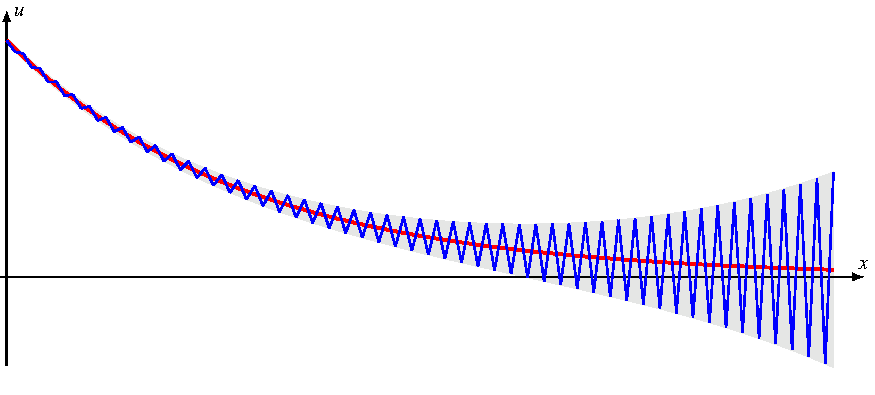
\includegraphics{learning/compmod.pdf}
\caption{Exakte Lösung (rot) und numerische Lösung (blau)
der Differentialgleichung
\eqref{burgers:expo}
unter Verwendung symmetrischer Differenzenquotienten.
Der Computational Mode äussert sich im exponentiellen Anwachsen
alternierender Fehler mit grösser werdendem $x$.
\label{burgers:compmod}}
\end{figure}

Die zweite Lösung $\lambda_-$ ist negativ und $|\lambda_-|>1$ für $h$
klein genug.
Die Gleichung~\ref{burgers:diffgl} hat also eine zusätzliche Lösung
$u_i=u_0\lambda_-^i$ mit alterniernden Vorzeichen, die sehr schnell anwächst.
Wir können wie bei $\lambda_+$ auch den Grenzwert für beliebig feine
Diskretisierung bestimmen.
Da das Vorzeichen dieser Lösung mit jedem Schritt wechselt, untersuchen
wir nur die geraden Schritte.
Wir nehmen wieder $h=x/2n$ und berechnen den Grenzwert
\[
\lim_{n\to\infty}
u_0
\biggl(
1+\frac{x}{2n}+\dots
\biggr)^{2n}
=
u_0e^x.
\]
Die Lösung wächst also exponentiell schnell an.

Die Lösung der Differentialgleichung ist eine Linearkombination
\[
u_i = a_+\lambda_+^i + a_-\lambda_-^i,
\]
deren Koeffizienten aus Anfangswerten bestimmt werden müssen.
Für fast alle Anfangswerte ist unvermeidbar, dass sich der
Koeffizient $a_-$ als von $0$ verschieden herausstellt, auch
wenn er sehr klein ist.
Weil $\lambda_-^i$ exponentiell schnell anwächst wird der Summand
$a_-\lambda_-^i$ immer früher oder später die numersiche Lösung dominieren,
wie dies auch in Abbildung~\ref{burgers:compmod} dargestellt ist.

Diese Lösung ist einzig entstanden durch den Versuch, mit Hilfe zusätzlicher
Funktionswerte das numerische Verfahren zu verbessern.
Dabei ist die Ordnung der Differenzengleichung grösser geworden und damit
sind neue Lösungen entstanden.

\subsubsection{Gleichung von Burgers und Computational Mode}
\begin{figure}
\centering
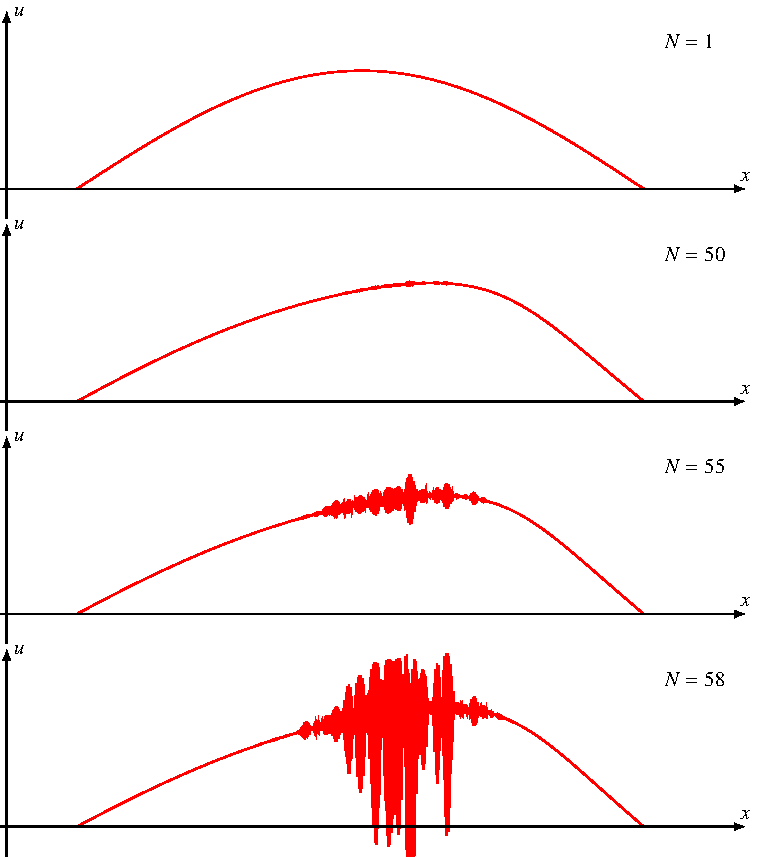
\includegraphics{learning/burgerwave.pdf}
\caption{Entwicklung des Computational Mode in einer Simulation
der Differenzengleichung \eqref{burgers:diffgleichung}.
Im obersten Graphen sieht man die Anfangsbedingung, die Funktion $\sin x$
zwischen $0$ und $2\pi$.
Bei Iteration $N=50$ kann man bereits erkennen, wie sich der Computational
Mode auszuwirken beginnt, die nachfolgend gezeigten Iterationen sind
unbrauchbar.
\label{burgers:burgerwave}}
\end{figure}
Das Problem des Computational Mode tritt auch bei der Gleichung von Burgers
auf.
Wir verwenden eine zweidimensionale Diskretisation $(t_i, x_j)$ mit
Schrittweite $h$.
Die asymmetrischen Differenzenquotienten
\[
\frac{\partial u(t_i,x_j)}{\partial t}
\simeq
\frac{u_{i+1,j} - u_{i,j}}{2h}
\qquad\text{und}\qquad
\frac{\partial u(t_i, x_j)}{\partial x}
\simeq
\frac{u_{i,j+1} - u_{i,j}}{2h}
\]
sind nicht wirklich repräsentativ für den Gitterpunkt $(i,j)$.
In die Gleichung geht zusätzlich zu den Ableitungen auch noch der
Funktionswert $u_{ij}$, was unterstreicht, dass wir die Ableitungen
möglichst genau an der Stelle $(i,j)$ bestimmen können müssen.

Die besser geeigneten symmetrischen Differenzenquotienten 
\[
\frac{\partial u(t_i,x_j)}{\partial t}
\simeq
\frac{u_{i+1,j} - u_{i-1,j}}{2h}
\qquad\text{und}\qquad
\frac{\partial u(t_i, x_j)}{\partial x}
\simeq
\frac{u_{i,j+1} - u_{i,j-1}}{2h}
\]
führen auf die nichtlineare Differenzengleichung
\begin{equation}
u_{i+1,j}
= 
u_{i-1,j}
+
h
u_{ij}\frac{u_{i,j+1}-u_{i,j-1}}{h}
=
u_{i-1,j}
+
u_{ij}(u_{i,j+1}-u_{i,j-1}),
\label{burgers:diffgleichung}
\end{equation}
die ebenfalls mindestens zweiter Ordnung ist.
Auch sie zeigt den Computational Mode, wie man zum Beispiel auch
in numerischen Experimenten sehen kann (Abbildung~\ref{burgers:burgerwave}).





